\section{Data Retrieval}
Die Aufgabe im Bereich Data Retrieval war es die zum einen die Daten aus der Datenbank auszulesen und diese mit einem virtuellen Notebook zu visualisieren.

Die Beschaffung und Auswertung der Daten mit Apache Zeppelin übernahm Julian Ruppel.
Johannes Weber bereitete die Daten mit Python auf und visualisierte sie in einem Jupyter Notebook.
\subsection{Data Retrieval mit Apache Zeppelin}
Apache Zeppelin bringt standardmäßig einige nützliche Funktionen mit, die es für die Datenauswertung interessant machen. Dazu zählen u.A.:
\begin{itemize}
	\item SQL via JDBC inkl. PostgreSQL Support
	\item Interaktive Diagramme über Formulargeneriung und Pivot-Charts
	\item Frei konfigurierbare Anordnung der Diagramme im Notebook
	\item Versionsverwaltung für Notebooks um verschiedene Stände abzuspeichern und schnell zwischen Versionen zu wechseln
\end{itemize}

Über den Befehl \shellcmd{/bin/zeppelin.sh} startet Zeppelin und ist standardmäßig im Browser über den Port 8080 erreichbar. Die gesamte Konfiguration, Entwicklung und Ausführung des Notebooks erfolgt im Web. Letztlich ist ein Notebook ein Kanvas in den man Kacheln erstellen und verwalten kann. Jede Kachel besteht aus 3 integralen Bestandteilen:
\begin{itemize}
	\item \textbf{Code} der mittels der vielen Interpreter die Daten läd, die angezeigt werden sollen, z.B. SQL.
	\item \textbf{Konfiguration} der Visualisierung. Dazu zählen verschiedene Diagrammtypen und -konfigurationen sowie generierte Formularfelder. 
	\item \textbf{Diagramm} welches die Daten responsiv visualisiert oder eine schlichte Tabelle um die Daten darzustellen.
\end{itemize}

Sobald der Code ausgeführt wird, egal ob manuell oder per automatischen Zyklus, wird das Diagramm in der Kachel aktualisiert.\linebreak
Leider ist die Auswahl an Diagrammtypen und deren Flexibilität und Erfassbarkeit abhängig von den Daten sehr begrenzt. Standardmäßig gibt es nur eine schlichte Tabelle, Balken-, Flächen-, Linien- und Punktdiagramm die relativ starr sind. Da erweiterte Visualisierungen wie Heatmaps und Karten noch in der Entwicklung sind ist die Auswertung auf die oben genannten Typen begrenzt. Zudem ist die maximale Anzahl an Datensätzen die dargestellt bzw. visualisiert werden könne auf 102400 begrenzt. Nichts desto trotz wurde ein beispielhaftes Notebook erstellt:

\begin{figure}[t] 
	\centering
	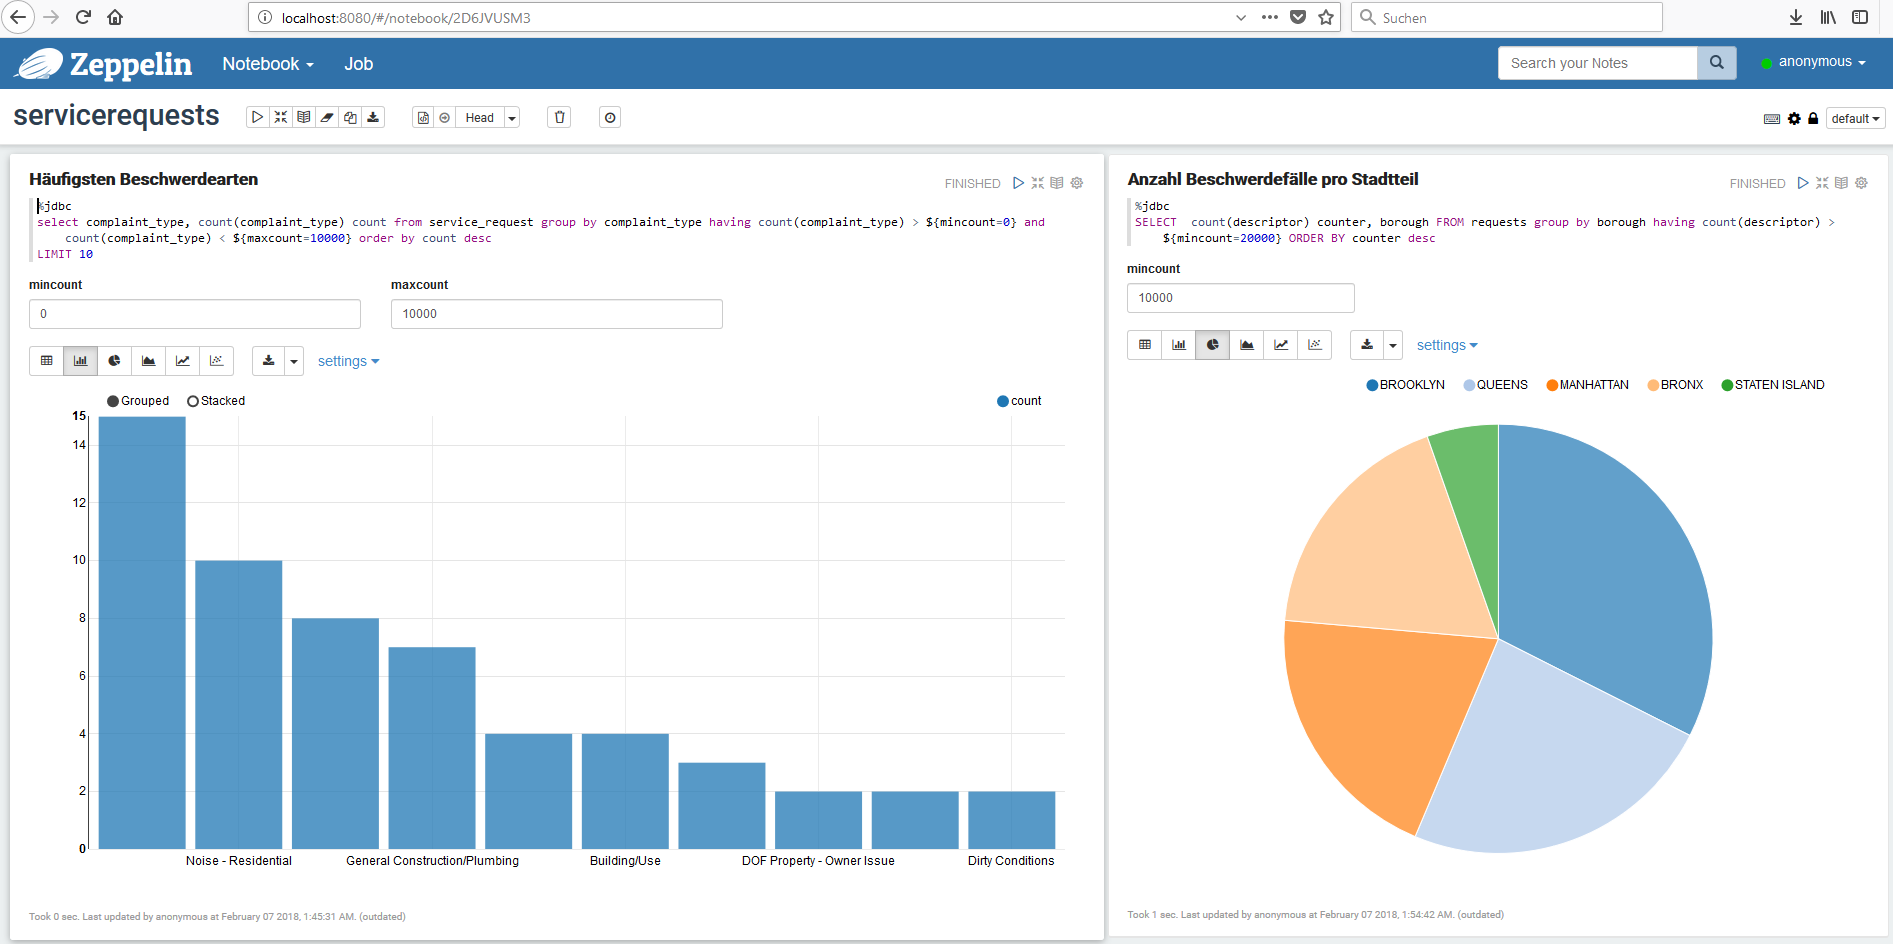
\includegraphics[width=\linewidth]{dualComplainChart.png}
	\caption[Ausschnitt des Notebooks]{Ausschnitt des Notebooks}
	\label{fig:zeppelin1}
\end{figure}
\begin{figure}[h] 
	\centering
	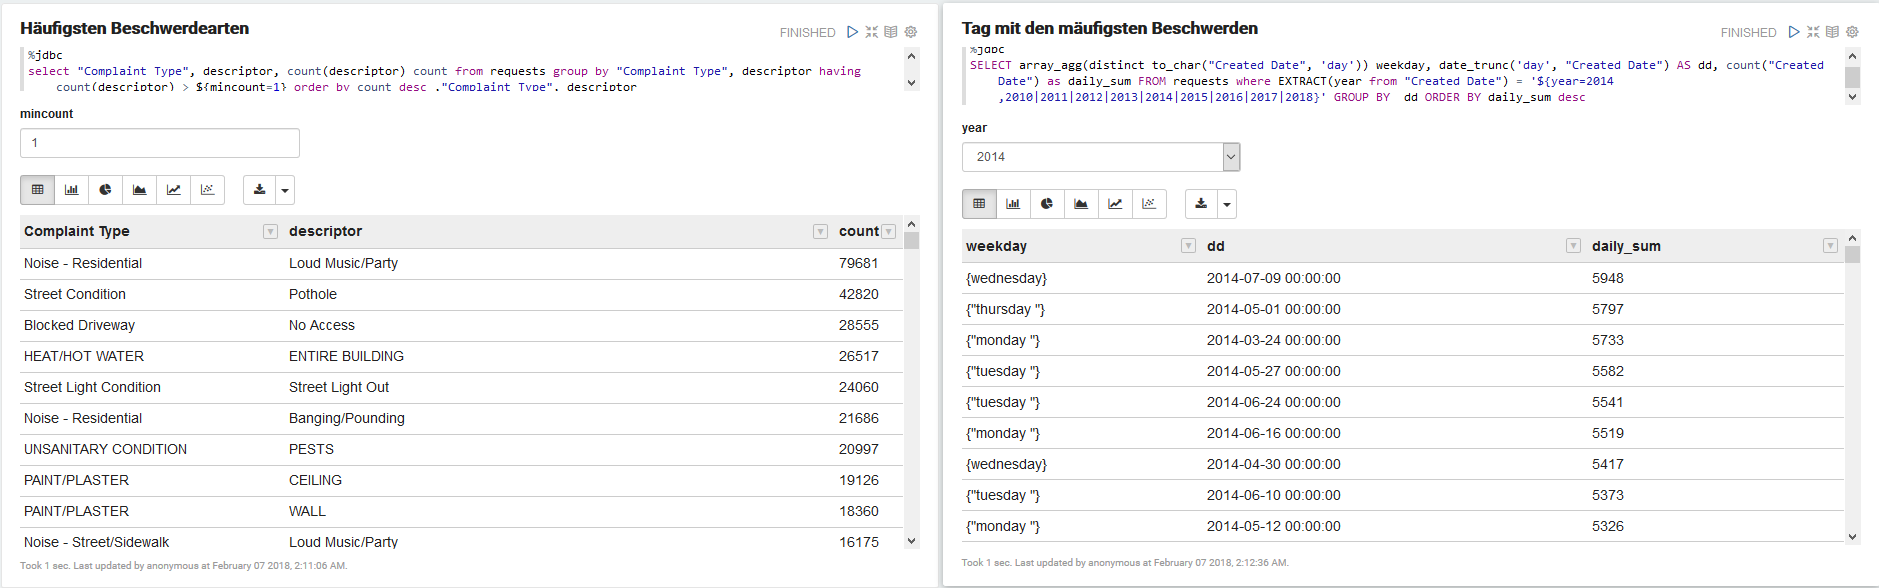
\includegraphics[width=\linewidth]{dualComplainDaychart.png}
	\caption[Ausschnitt des Notebooks]{Ausschnitt des Notebooks}
	\label{fig:zeppelin2}
\end{figure}
\begin{figure}[h] 
	\centering
	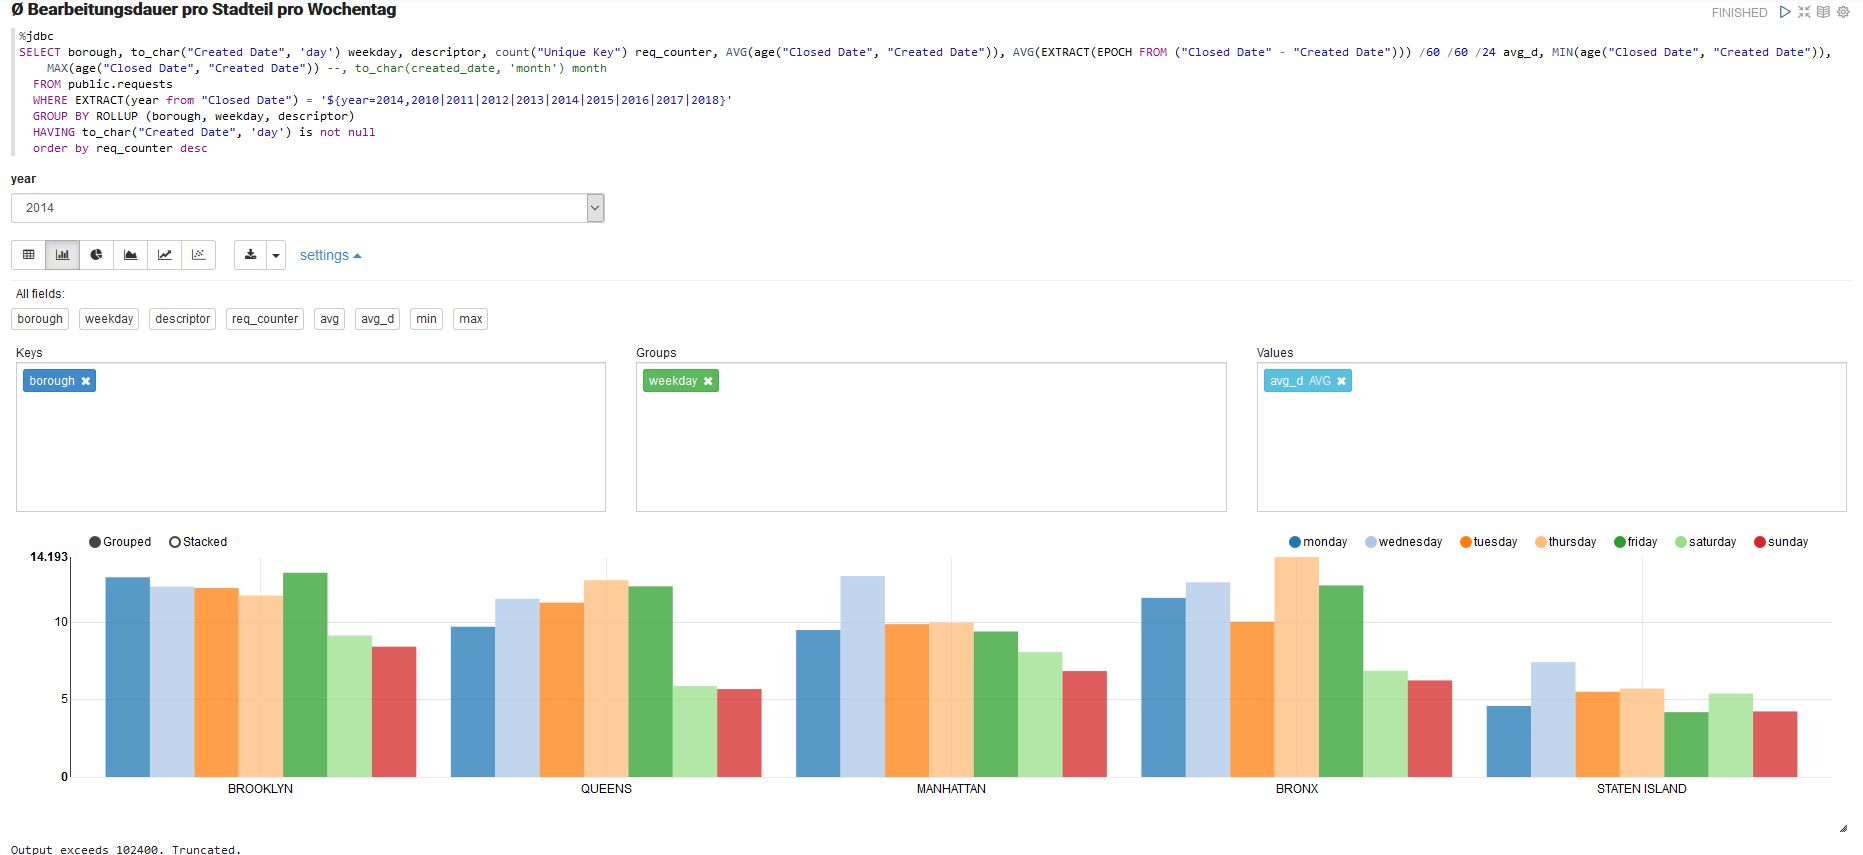
\includegraphics[width=\linewidth]{comByRegion.png}
	\caption[Ausschnitt des Notebooks]{Ausschnitt des Notebooks}
	\label{fig:zeppelin3}
\end{figure}



\subsection{Data Retrieval mit Jupyter}
Das Jupyter Notebook bietet die Möglichkeit mit \textit{Magic-Commands} direkt aus dem Notebook heraus
eine Verbindung mit der Datenbank aufzubauen und \ac{SQL} Statements abzusetzen.
Einfache Tabellen werden direkt in Jupyter visualisiert wohingegen komplexere Visualisierungen wie \zb{}
Balkendiagramme oder Geo Plots mit Python Bibliotheken dargestellt werden müssen.
Für die Darstellung in Jupyter werden sog. \textit{Widgets} installiert und aktiviert.


Folgende Python Bibliotheken wurden installiert um \ac{SQL} Statements in Jupyter ausführen und visualisieren zu können.
\begin{itemize}
  \item ipython-sql
  \item sqlalchemy (wird von ipython-sql benötigt)
  \item bokeh
  \item gmaps
\end{itemize}

Mit \code{ipython-sql} werden \ac{SQL} \textit{Magic-Command} in Jupyter aktiviert.
\code{ipython-sql} nutzt \code{sqlalchemy} um sich mit der Datenbank zu verbinden.
Ein abgesetztes \ac{SQL} Statement lässt sich entweder direkt in Jupyter ausgeben
oder einer beliebigen Variable zuordnen die dann weiterverarbeitet werden kann.


 \code{bokeh} ist eine mächtige Python Bibliothek um viele Arten der Visualisierung umzusetzen
 wie \zb{} Balkendiagramme, Scatter Plots, Geo Maps oder Zeitreihen.


 Die Visualisierung von Geo Daten erfolgt mit der Bibliothek \code{gmaps}.
 Diese greift auf die Karten von Google Maps zu erlaubt es die Geo Daten in einem Layer über einen
 beliebigen Kartenausschnitt zu legen.
 Der Vorteil von \code{gmaps} gegenüber \code{bokeh} ist
 zum einen die Nutzung des Kartenmaterials von Google aber auch die interaktive Nutzung
 des Kartenauschnitts mit \zb{} StreetView.


Folgende Fragestellungen wurden im Rahmen von Data Retrieval beantwortet.

\begin{enumerate}
  \item Zeige alle Beschwerdetypen die häufiger als 400 aber seltener als 8000 Mal gemeldet wurden?
  \item Wie lautet die Beschreibung der häufig vorkommenden Service Requests?
  \item An welchen Orten von New York City wurden Service Request vom Typ 'Noise - Residential' abgesetzt?
  \item Wieviele Service Requests sind im Jahr 2017 eingegangen? Gruppiert nach Tag und Sortiert nach dem Erstellungsdatum.
\end{enumerate}

Nachfolgender Abschnitt listet die \ac{SQL} Statements zu jeder Fragestellung sowie ein dazugehöriges Beispiel.


\textbf{zu 1.}
\newline
\sql{SELECT complaint\_type, COUNT(complaint\_type) FROM service\_request GROUP BY complaint\_type HAVING COUNT(complaint\_type) > 400 AND COUNT(complaint\_type) < 8000}

\bildhochkant{select_1.png}{Tabelle mit allen Beschwerdetypen}{srt}{eigene Darstellung}

\textbf{zu 2.}
\newline
\sql{SELECT descriptor, COUNT(descriptor) FROM service\_request  WHERE descriptor IS NOT NULL GROUP BY descriptor ORDER BY count DESC}

\bild{select_2.png}{Auszug aus den meisten Service Requests}{toprequests}{eigene Darstellung}{0.75}

\textbf{zu 3.}
\newline
\sql{SELECT longitude, latitude FROM service\_request WHERE complaint\_type = 'Noise - Residential' and latitude IS NOT NULL and longitude IS NOT NULL}

\bild{select_3.png}{Heatmap der Lärmquellen in New York}{rnnyc}{eigene Darstellung}{0.75}

\textbf{zu 4.}
\newline
\sql{SELECT date\_trunc('day', created\_date) AS dd, COUNT(created\_date) as daily\_sum FROM service\_request where EXTRACT(year from created\_date) = '2017' GROUP BY dd ORDER BY date\_trunc('day', created\_date)}

\bild{select_4.png}{Timeline aller Service Requests in 2017}{sr2017}{eigene Darstellung}{0.75}

